%!TEX root = ../../main.tex

\graphicspath{{../../figures/appendix/}}

\chapter{Simulations}
\label{ch:appendix_simulation}

\newpage

\section{Spot and cluster simulations}
\label{sec:appendix_simulations_spots}

\vfill

\noindent
Figure~\ref{fig:spots_mosaic} is a sample of simulated images of spots.
We modulate the number of spots and the intensity of the noise for each image.

\vfill

\begin{figure}[h]
    \centering
    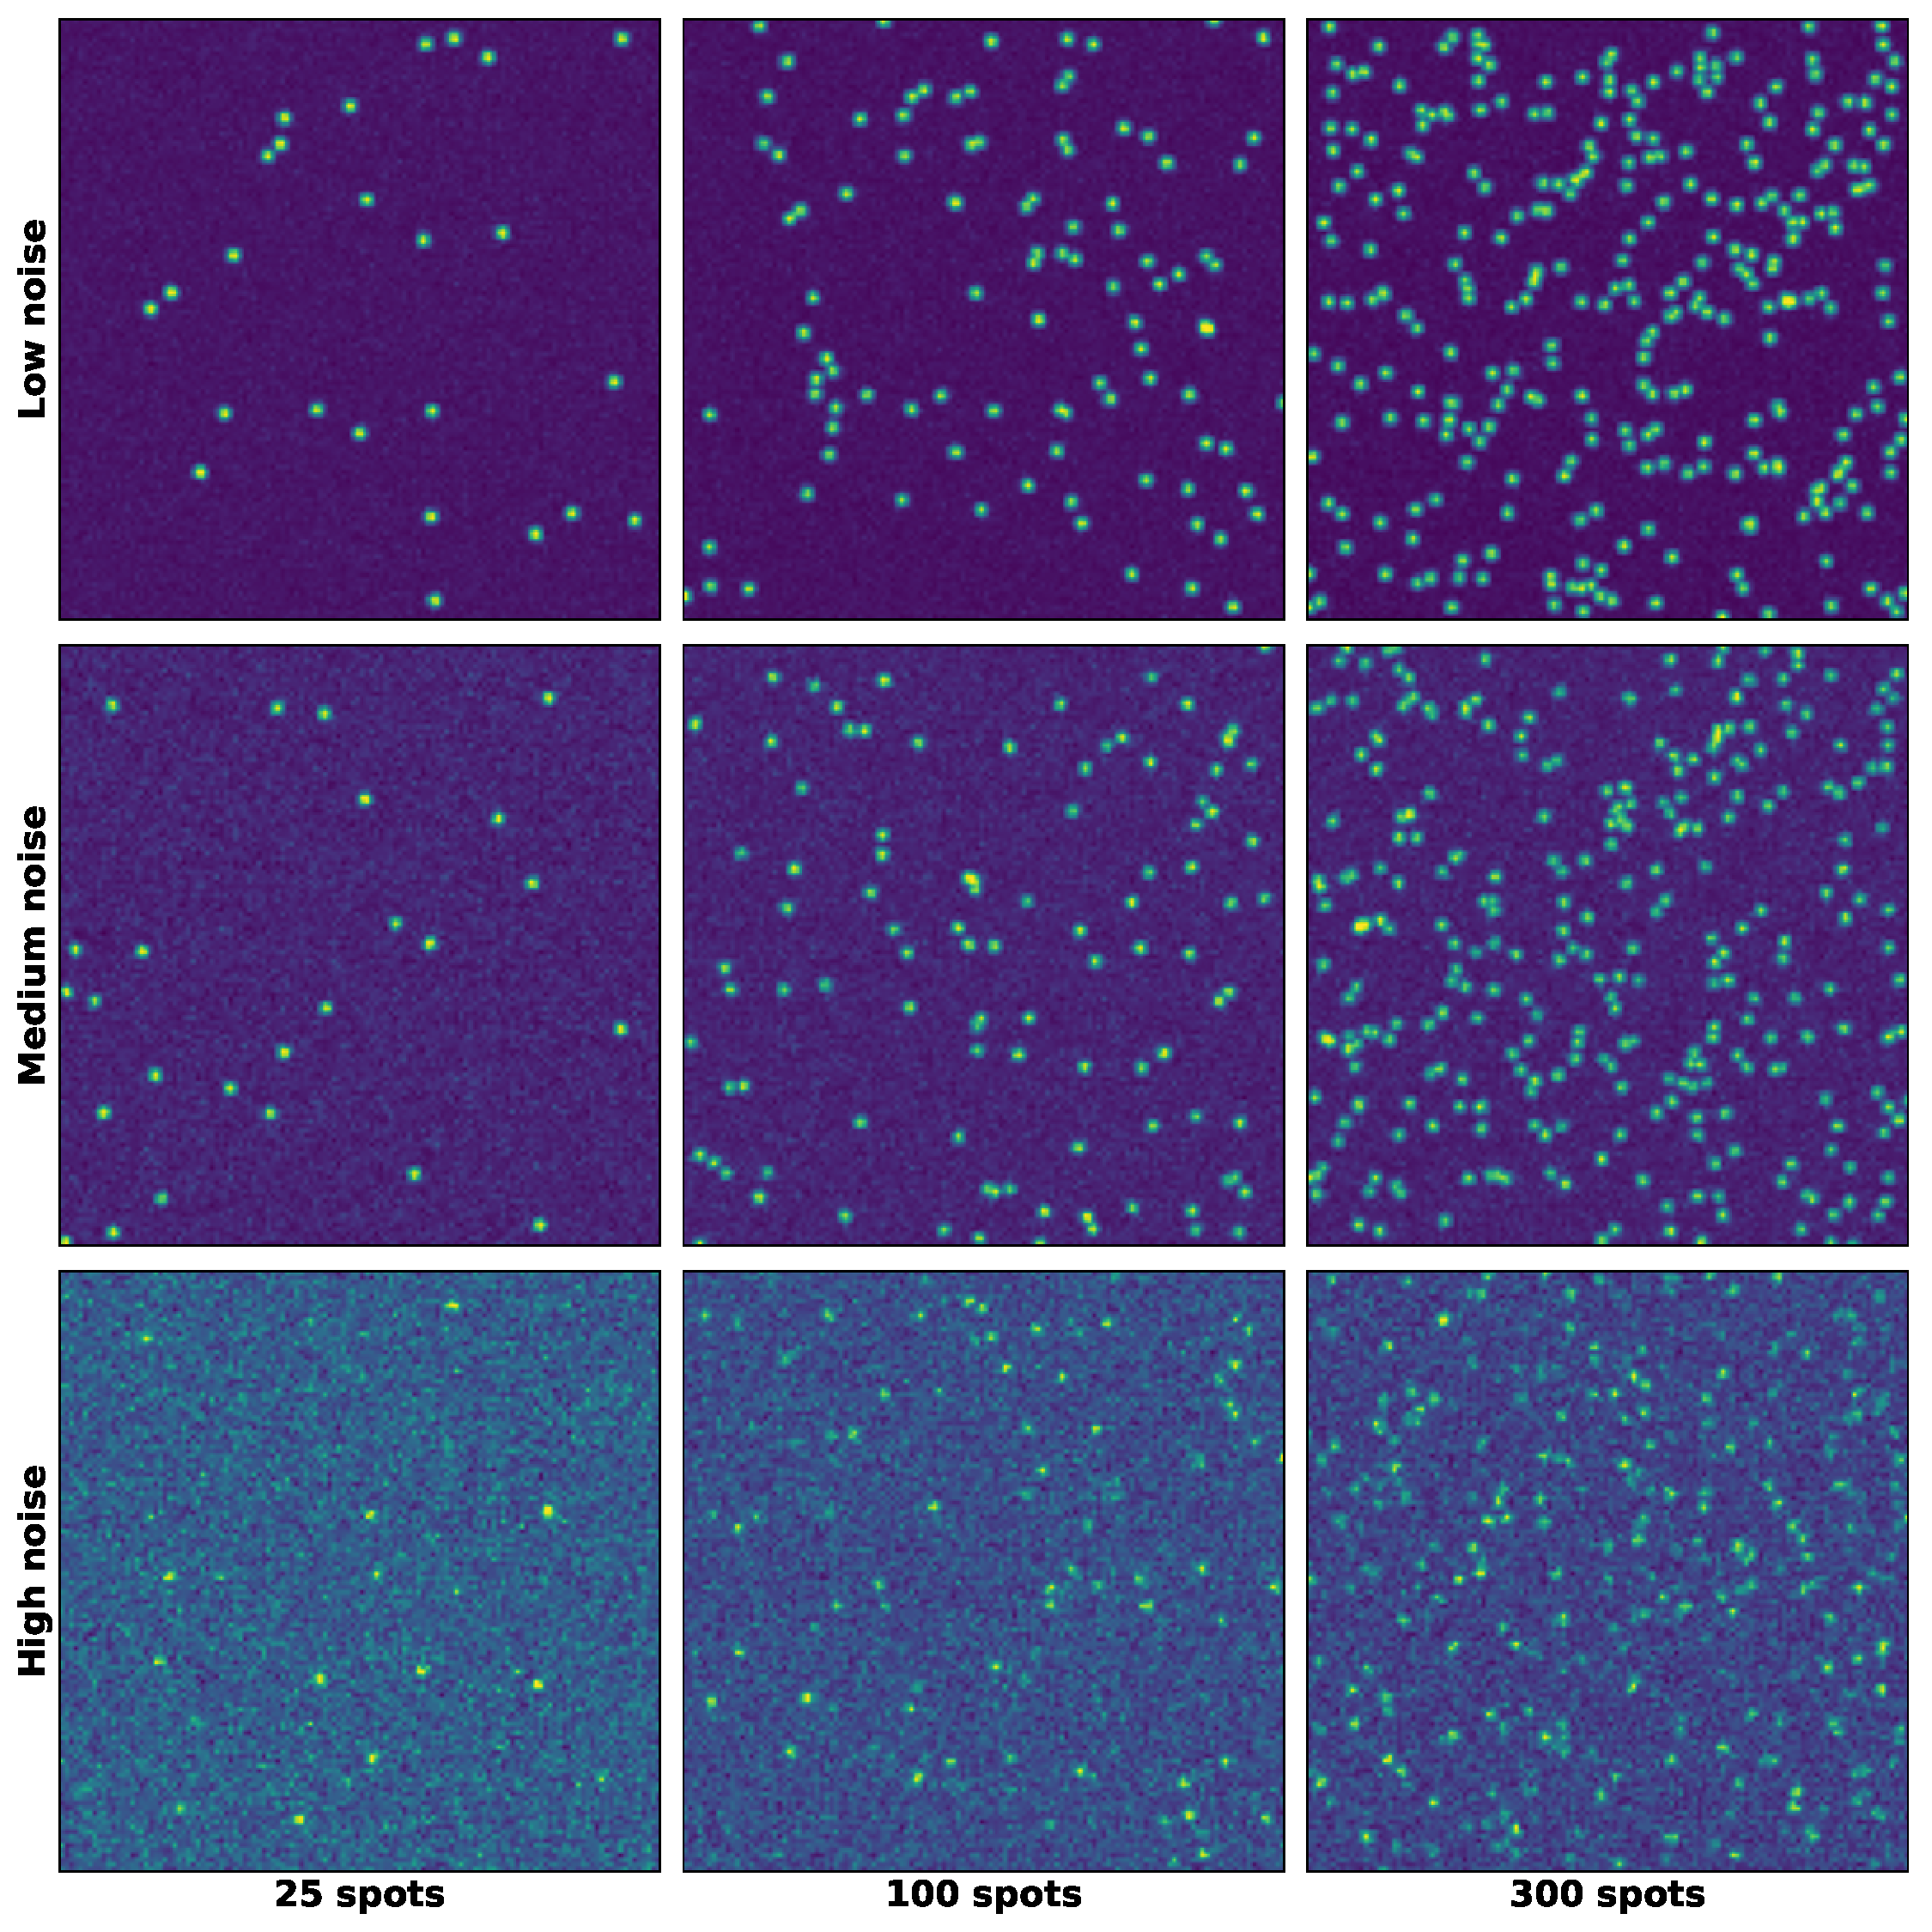
\includegraphics[width=\textwidth]{figures/appendix/spots_mosaic}
    \caption[Spot simulations under different noise regimes]{Simulations of spots under different noise regimes}
    \label{fig:spots_mosaic}
\end{figure}

\newpage

\null
\vfill

\noindent
Figure~\ref{fig:cluster_mosaic} use the same logic but with a unique cluster of spots simulated in the center.
This time, we modulate the number of spots inside the cluster.

\vfill

\begin{figure}[h]
    \centering
    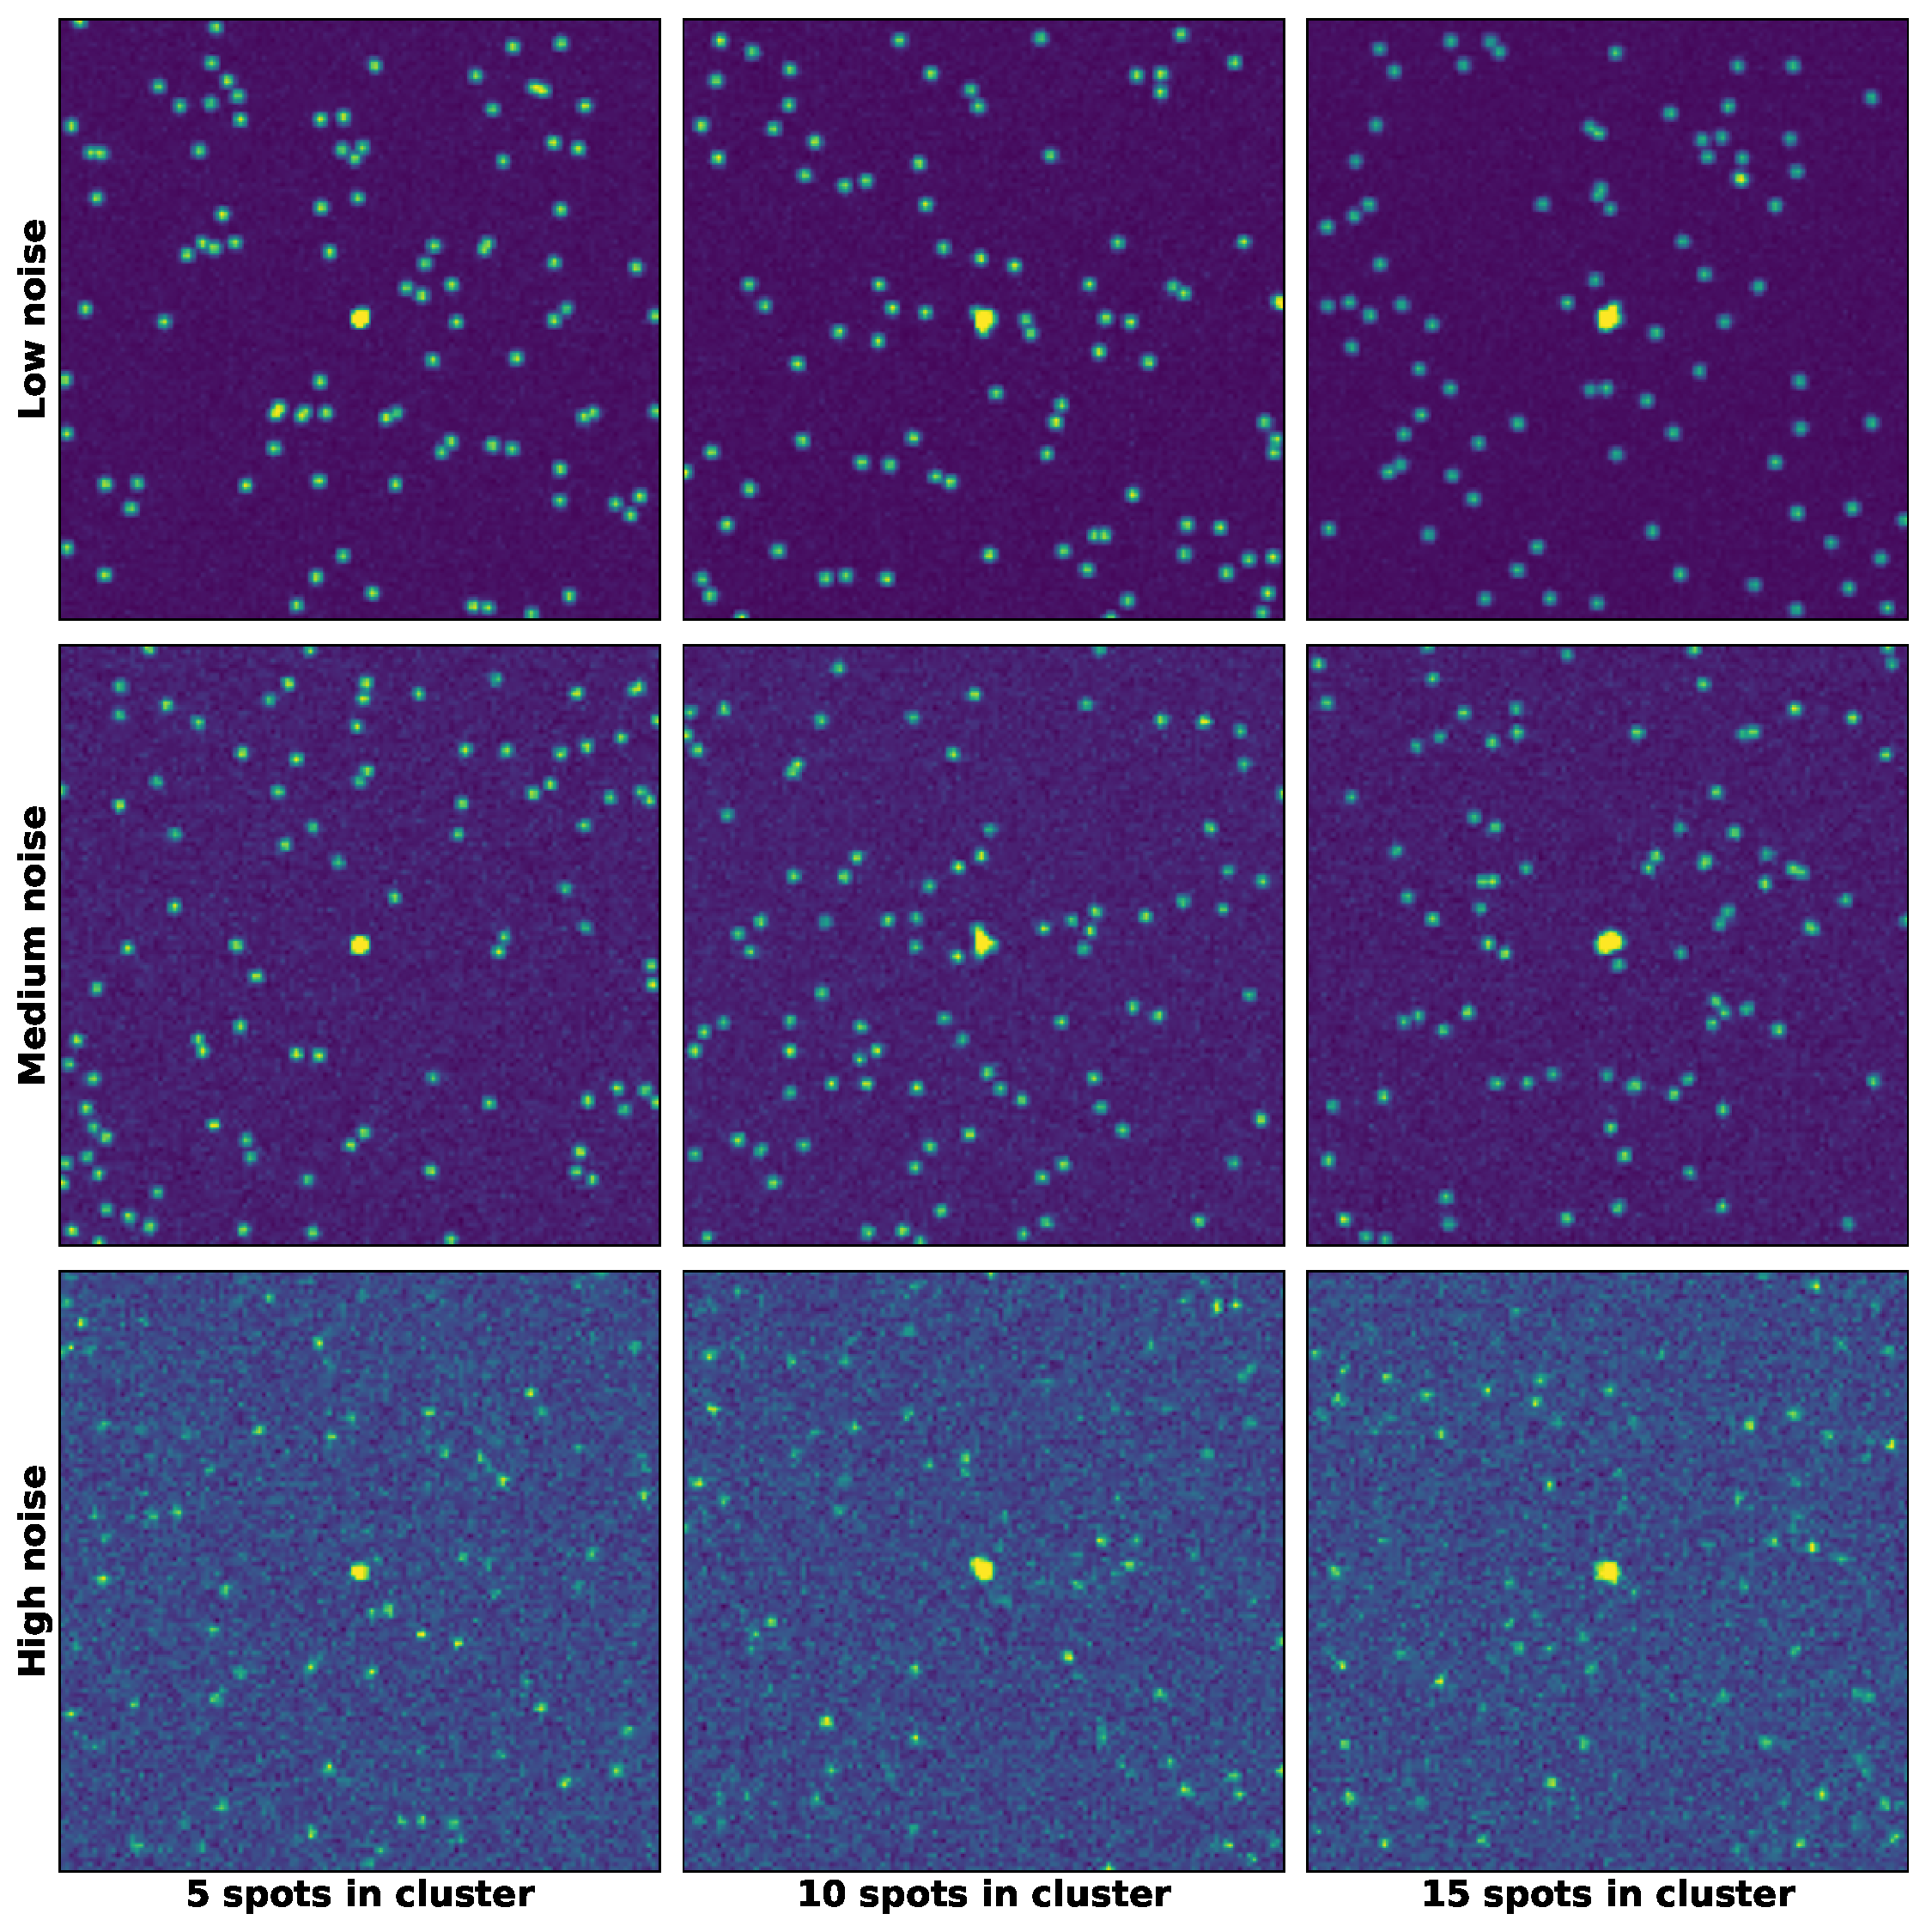
\includegraphics[width=\textwidth]{figures/appendix/cluster_mosaic}
    \caption[Cluster simulations under different noise regimes]{Simulations of cluster under different noise regimes}
    \label{fig:cluster_mosaic}
\end{figure}

\newpage

\section{Localization pattern simulations}
\label{sec:appendix_simulations_pattern}

\vfill

\begin{figure}[h]
    \centering
    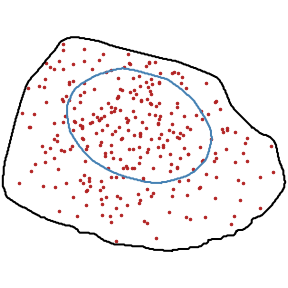
\includegraphics[width=0.2\textwidth]{figures/appendix/random_1_300}
    \caption[Random spot simulations]{Simulations of random spots}
    \label{fig:random_1_300}
\end{figure}

\vfill

\noindent
Figure~\ref{fig:random_1_300} is an example of random pattern with 300 simulated spots.
On the contrary, in figures~\ref{fig:all_patterns_1} and~\ref{fig:all_patterns_2} we can observe localized patterns, with 300 simulated spots as well, but different pattern strengths (10\%, 50\% and 90\% of localized spots).

\vfill

\begin{figure}[h]
    \centering
    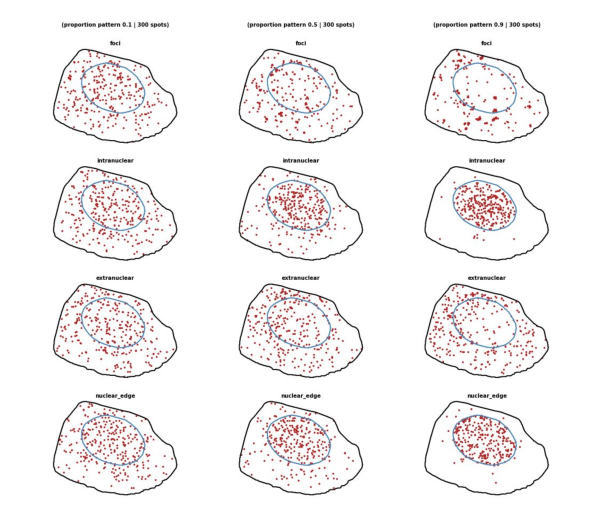
\includegraphics[width=\textwidth]{figures/appendix/all_patterns_1}
    \caption[Localization pattern simulations (first part)]{Simulations of localization patterns (first part)}
    \label{fig:all_patterns_1}
\end{figure}

\newpage

\null
\vfill

\noindent
Because we visualize plots in 2D, some of these localization patterns (simulated in 3D) can be misleading.
In particular, visualized in 2D, cell edge pattern can appear similar to random pattern, and nuclear edge pattern looks like intranuclear one.
Same difficulties can arise when one manually annotate real cell images.

\vfill

\begin{figure}[h]
    \centering
    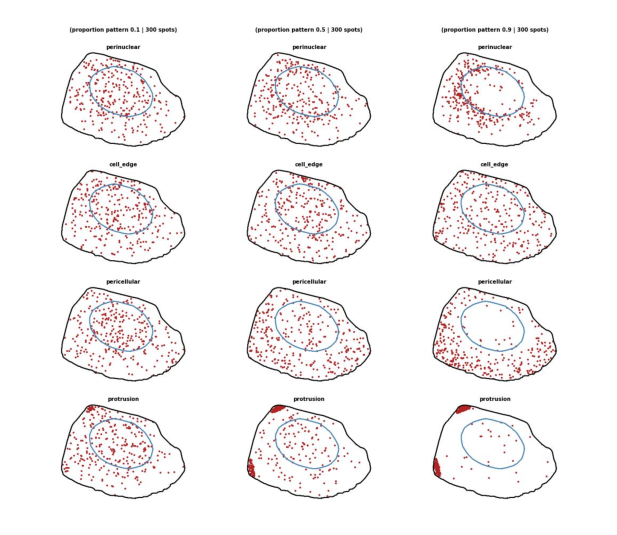
\includegraphics[width=\textwidth]{figures/appendix/all_patterns_2}
    \caption[Localization pattern simulations (second part)]{Simulations of localization patterns (second part)}
    \label{fig:all_patterns_2}
\end{figure}
